\documentclass[11pt]{article}
\usepackage[margin=2.0cm]{geometry}
\usepackage{booktabs}
\usepackage{amsmath}
\usepackage{amssymb}
\usepackage{enumitem}
\usepackage{array}
\usepackage{listings}
\usepackage{xcolor}
\usepackage{tikz}
\usepackage[T1]{fontenc}
\usepackage{lmodern}

\setlength{\parindent}{0pt}
\setlength{\parskip}{3.6pt}
\newcommand{\code}[1]{\texttt{#1}}
\newcommand{\hr}{\vspace{2pt}\hrule\vspace{6pt}}
\renewcommand{\arraystretch}{1.12}

\definecolor{kw}{RGB}{0,90,160}
\definecolor{cmt}{RGB}{110,110,110}
\lstdefinestyle{vhdl}{
  language=VHDL, basicstyle=\ttfamily\footnotesize,
  keywordstyle=\color{kw}\bfseries, commentstyle=\color{cmt}\itshape,
  showstringspaces=false, columns=fullflexible, breaklines=true,
  frame=leftline, framesep=6pt, xleftmargin=8pt, aboveskip=6pt, belowskip=6pt
}
\lstset{style=vhdl}

\begin{document}

\begin{center}
{\Large\bfseries EE\,362 --- Computer Organization Laboratory}\\[2pt]
{\large\bfseries Lab 2 --- Solution}\\[2pt]
{\itshape Master--Slave Flip-Flop and the N-Bit Register}\\[4pt]
Fall 2026 \quad$\cdot$\quad Lab TA: Gandhi Torres
\end{center}
\hr

Worked solution for \code{MSFlipFlop} and \code{RegN}. Read it after your own
attempt runs. Every number quoted here was measured with Quartus Prime Lite
25.1std and Questa on device \code{5CSEMA4U23C6}.

\vspace{4pt}\hr

\section*{1. Where the edge comes from}

Nobody designs an ``edge''. It falls out of two latches wired in opposition.

\begin{center}
\begin{tabular}{lll}
\toprule
& master (\code{En = not Clk}) & slave (\code{En = Clk}) \\
\midrule
\code{Clk = '0'} & \textbf{transparent}, follows \code{D} & holding \\
\code{Clk = '1'} & holding & \textbf{transparent}, copies the master \\
\bottomrule
\end{tabular}
\end{center}

\textbf{The two latches are never open at the same time.} That is the whole
mechanism. While the clock is low, \code{D} can reach the master but no further.
The instant the clock rises, the master freezes on whatever \code{D} was, and the
slave opens and copies it. So \code{Q} can only change at a rising edge.

\begin{center}
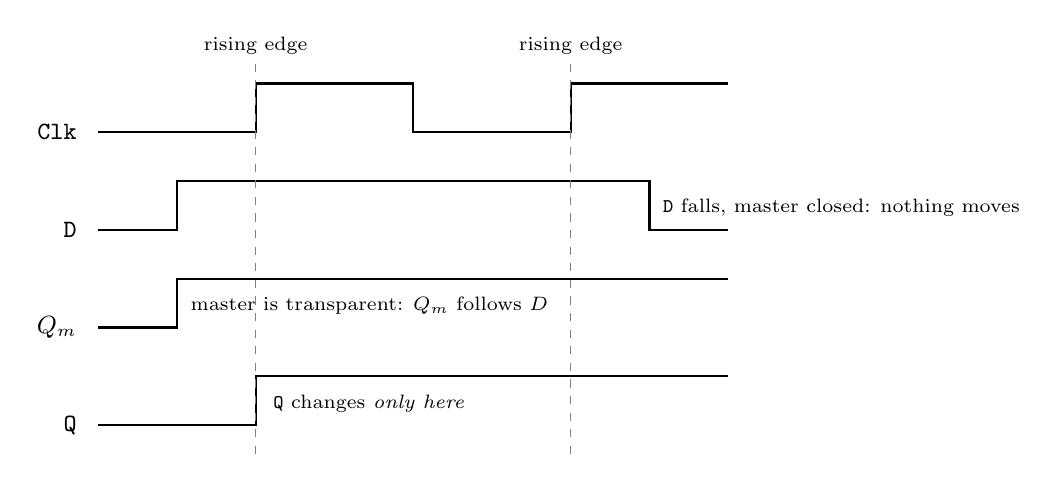
\begin{tikzpicture}[x=1.0cm, y=0.62cm]
  \node[left] at (-0.15, 0) {\small\code{Clk}};
  \draw[thick] (0,0) -- (2,0) -- (2,1) -- (4,1) -- (4,0) -- (6,0) -- (6,1) -- (8,1);
  \node[left] at (-0.15,-2) {\small\code{D}};
  \draw[thick] (0,-2) -- (1,-2) -- (1,-1) -- (7,-1) -- (7,-2) -- (8,-2);
  \node[left] at (-0.15,-4) {\small$Q_m$};
  \draw[thick] (0,-4) -- (1,-4) -- (1,-3) -- (8,-3);
  \node[left] at (-0.15,-6) {\small\code{Q}};
  \draw[thick] (0,-6) -- (2,-6) -- (2,-5) -- (8,-5);
  \foreach \x in {2,6} \draw[dashed,gray] (\x,1.4) -- (\x,-6.6);
  \node[above] at (2,1.4) {\scriptsize rising edge};
  \node[above] at (6,1.4) {\scriptsize rising edge};
  \node[right,font=\scriptsize] at (1.05,-3.55) {master is transparent: $Q_m$ follows $D$};
  \node[right,font=\scriptsize] at (2.1,-5.55) {\code{Q} changes \emph{only here}};
  \node[right,font=\scriptsize] at (7.05,-1.55) {\code{D} falls, master closed: nothing moves};
\end{tikzpicture}
\end{center}

\subsection*{Equations --- Lab 1's latch, twice, with different enables}

\begin{align*}
\text{master} \quad & Q_m^{+} = \overline{Clr}\cdot\left( \overline{Clk}\cdot D + Clk\cdot Q_m \right)\\
\text{slave}  \quad & Q^{+}   = \overline{Clr}\cdot\left( Clk\cdot Q_m + \overline{Clk}\cdot Q \right)
\end{align*}

Both are last week's equation $Q^{+} = \overline{Clr}(En\cdot D + \overline{En}\cdot Q)$.
The only change is what is connected to $En$: $\overline{Clk}$ for the master,
$Clk$ for the slave. \textbf{You wrote no new equation this week.}

\section*{2. \code{MSFlipFlop} --- the structural build}

\begin{lstlisting}
architecture structural of MSFlipFlop is
    signal Qm   : std_logic;
    signal ClkN : std_logic;
begin
    ClkN <= not Clk;

    MASTER : entity work.TransLatch
        port map (D => D,  En => ClkN, Clr => Clr, Q => Qm);

    SLAVE  : entity work.TransLatch
        port map (D => Qm, En => Clk,  Clr => Clr, Q => Q);
end architecture structural;
\end{lstlisting}

Three things to notice, because each is a habit for the rest of the course:

\begin{itemize}[leftmargin=1.6em,itemsep=2pt]
\item \textbf{This is structural VHDL in the strict sense.} Two \emph{components}
joined by signals --- not operators. From here to Lab 12 this is how everything is
built.
\item \textbf{Named association everywhere} (\code{D => D}, \code{En => ClkN}).
The two instances differ only in what is connected to \code{En} and \code{D}; with
positional maps that difference would be invisible.
\item \textbf{\code{Qm} is the wire between them}, and it is the signal to add to
your waveform. It is the only place the mechanism is visible.
\end{itemize}

\subsection*{Why \code{Clr} must reach \emph{both} latches}

\code{Clr} is connected to the master and to the slave. Clear only the slave and
this happens:

\begin{enumerate}[leftmargin=2em,itemsep=1pt]
\item \code{Clr} clears the slave, so \code{Q} goes to 0. It looks correct.
\item But the master still holds the old value --- nothing cleared it.
\item At the very next rising edge the slave copies the master, and the old value
comes straight back.
\end{enumerate}

\textbf{The clear appears to undo itself one cycle later.} Try it deliberately
once your design works: disconnect \code{Clr} from the master, and watch check~7
of the testbench fail while check~6 still passes.

\section*{3. \code{RegN} --- the same table, one lab later}

\subsection*{Specification --- Table T}

\begin{center}
\begin{tabular}{c|ccc|c|l}
\toprule
\# & \code{Rst} & \code{Ld} & \code{Clk} & $Q^{+}$ & note \\
\midrule
0 & 1 & -- & -- & \textbf{0} & asynchronous reset, dominates \\
1 & 0 & -- & not $\uparrow$ & $\mathbf{Q}$ & hold between edges \\
2 & 0 & 0 & $\uparrow$ & $\mathbf{Q}$ & edge arrives, but not loading \\
3 & 0 & 1 & $\uparrow$ & $\mathbf{D}$ & load \\
\bottomrule
\end{tabular}
\end{center}

\begin{align*}
\text{(1) at the edge} \quad & Q_i^{+} = \overline{Rst}\cdot\left( Ld\cdot D_i + \overline{Ld}\cdot Q_i \right)\\
\text{(2) observation} \quad & \text{identical to Lab 1 with } En \to Ld,\ Clr \to Rst
   \quad\text{[same equation, new names]}\\
\text{(3) VHDL} \quad & \text{nested \code{if} inside \code{rising\_edge}}
\end{align*}

Row 1 is new and it is free: between edges the process does not run at all, so
\code{Q} holds without any code being written for it.

\subsection*{The code}

\begin{lstlisting}
entity RegN is
    generic ( N : positive := 32 );
    port (
        D   : in  std_logic_vector(N - 1 downto 0);
        Clk : in  std_logic;
        Ld  : in  std_logic;
        Rst : in  std_logic;
        Q   : out std_logic_vector(N - 1 downto 0)
    );
end entity RegN;

architecture behavioral of RegN is
begin
    process (Clk, Rst)
    begin
        if Rst = '1' then
            Q <= (others => '0');       -- row 0, asynchronous
        elsif rising_edge(Clk) then
            if Ld = '1' then
                Q <= D;                 -- row 3
            end if;
            -- row 2 (edge, Ld low) is the missing else
        end if;
    end process;
end architecture behavioral;
\end{lstlisting}

\subsection*{Three details that are not decoration}

\textbf{(a) \code{Rst} is tested before the edge, and outside it.} That is what
makes it asynchronous: the branch is reachable without a clock event. Writing
\code{if rising\_edge(Clk) then if Rst = '1' ...} gives a \emph{synchronous} reset,
which is a different circuit and contradicts row 0.

\textbf{(b) \code{Ld} goes in a nested \code{if}, not on the \code{elsif}.} These
simulate identically:

\begin{lstlisting}
elsif rising_edge(Clk) and Ld = '1' then   -- works, but do not write it
elsif rising_edge(Clk) then                -- write this
    if Ld = '1' then ...
\end{lstlisting}

The second keeps the edge test as the \emph{only} condition on the \code{elsif},
which is the pattern every synthesiser recognises as ``clocked process''. The
first form makes \code{Ld} part of the clock expression, and some tools will build
gated-clock logic from it --- a real hardware problem, not a style opinion.

\textbf{(c) The missing \code{else} is row 2 again.} Same mechanism as Lab 1: no
assignment means hold. Last week it produced a latch; this week, inside
\code{rising\_edge}, it produces a register with a load enable. \textbf{Identical
VHDL rule, different hardware, because of what surrounds it.}

\subsection*{The sensitivity list --- the rule changed this week}

\begin{center}
\begin{tabular}{lll}
\toprule
& Lab 1 (latch) & Lab 2 (register) \\
\midrule
rule & every signal the process \emph{reads} & the clock $+$ asynchronous controls, nothing else \\
list & \code{(Clr, En, D)} & \code{(Clk, Rst)} \\
why & level-sensitive: \code{D} matters continuously & edge-triggered: \code{D} matters only at the edge \\
\bottomrule
\end{tabular}
\end{center}

\code{Ld} and \code{D} are read only at the rising edge, and at that instant the
process is already awake because \code{Clk} changed. Adding them changes nothing
in simulation and nothing in hardware --- but it shows you applied last week's
rule without noticing that it moved.

\section*{4. The generic --- one entity, every width}

\begin{lstlisting}
DUT_R5  : entity work.RegN generic map (N => 5)
    port map (D => D5, Clk => Clk, Ld => Ld, Rst => Rst, Q => Q5);

DUT_R32 : entity work.RegN generic map (N => 32)
    port map (D => D32, Clk => Clk, Ld => Ld, Rst => Rst, Q => Q32);
\end{lstlisting}

\textbf{\code{generic map} comes first, and there is no semicolon between it and
\code{port map}.} They are one statement.

\textbf{If you forget \code{generic map} entirely}, you silently get the default
width of 32, and the error appears at the \emph{signal} you connected --- not at
the instance that is wrong. Expect to read an error that points somewhere
innocent; the cause is almost always a missing or wrong \code{generic map}.

Why this matters beyond this lab: Lab 6 needs 32 of these at 32 bits, Lab 7 needs
one at 32 bits for the program counter, and several labs need 5-bit registers for
register numbers. \textbf{One entity serves all of them.}

\section*{5. The testbench --- 20 checks, and what each one is for}

Three components are tested at once: \code{MSFlipFlop}, \code{RegN(5)} and
\code{RegN(32)}, all driven by the same clock and controls.

\begin{center}
\small
\begin{tabular}{c>{\raggedright\arraybackslash}p{6.6cm}>{\raggedright\arraybackslash}p{6.6cm}}
\toprule
\# & what it drives & what it catches \\
\midrule
1 & \code{Rst}/\code{Clr} asserted \textbf{mid-period}, with \code{Ld}=1 and data all ones
  & a reset that is really \textbf{synchronous} (it would wait for the edge) \\
2 & data set after a falling edge, then one rising edge
  & the register never loads at all \\
3 & \textbf{toggle \code{D} three times between two edges}
  & \textbf{a transparent latch instead of a flip-flop} \\
4 & the next rising edge after those toggles
  & capturing an \emph{earlier} value instead of the last one before the edge \\
5 & an edge with \code{Ld} = 0
  & a register that ignores its load enable (row 2) \\
6a/6b & load, then \code{Clr} mid-period
  & a clear that only acts at an edge \\
7 & the edge \emph{after} that clear
  & \textbf{\code{Clr} wired to the slave only} --- the value returns \\
\bottomrule
\end{tabular}
\end{center}

\subsection*{Two timing rules the testbench obeys, and your own must too}

\textbf{Stimulus changes after a falling edge; checks happen 1~ns after a rising
edge.}

\begin{lstlisting}
wait until falling_edge(Clk);      -- change inputs far from the edge
Dff <= '1'; D32 <= x"DEADBEEF";
wait until rising_edge(Clk);
wait for 1 ns;                     -- let the edge take effect, then check
checkff('1', "2. FF captured D at the edge");
\end{lstlisting}

\textbf{Why not change \code{D} on the rising edge?} That is a setup-time
violation. In simulation you get whichever value the delta-cycle ordering happens
to produce, and in hardware the flip-flop may capture either value or go
metastable. The result is meaningless either way, so never write it.

\textbf{Why check 1~ns \emph{after} the edge, not at it?} At the exact instant of
the edge the new value has not propagated yet, and you would read the old one.

\subsection*{The clock generator, and why it stops}

\begin{lstlisting}
clock_gen : process
begin
    while running loop
        Clk <= '0'; wait for PERIOD / 2;
        Clk <= '1'; wait for PERIOD / 2;
    end loop;
    wait;
end process clock_gen;
\end{lstlisting}

The \code{running} flag is set false by the stimulus process at the end. Without
it, \code{run -all} never finishes: the clock process always has something to do,
so simulation time advances forever.

\textbf{And a clock process with \emph{no} \code{wait} at all is worse:} it loops
at time zero without advancing time. The simulation looks frozen. It is not
frozen --- it is spinning. If Questa hangs at 0~ns, this is why.

\section*{6. Quartus evidence}

\subsection*{E1 --- Flow Summary, with the top level set to \code{RegN}}

\begin{center}
\begin{tabular}{ll}
\toprule
\textbf{Total registers} & \textbf{32} \\
Total pins & 67 \quad (32 in, 32 out, \code{Clk}, \code{Ld}, \code{Rst}) \\
Logic utilisation & 9 ALMs \\
Inferred latches & \textbf{0} \\
\bottomrule
\end{tabular}
\end{center}

\textbf{The register count is a correctness check, not a cost figure.} A 32-bit
register must report exactly \textbf{32} registers. Anything else means you
described something you did not intend: 64 usually means an accidental second
storage stage, and 0 means the clocked process is not clocked at all.

\textbf{Zero inferred latches}, in contrast to Lab 1, where the same missing
\code{else} produced a latch. Inside \code{rising\_edge} it produces a register.

Pin count 67: the two 32-bit vectors plus three single-bit controls ---
\textbf{control is narrow, data is wide}, now visible as a number.

\subsection*{E1 --- \code{MSFlipFlop} compiled on its own}

\begin{center}
\begin{tabular}{ll}
\toprule
Total registers & \textbf{0} \\
Inferred latches & \textbf{2} \quad (\code{Qm} and \code{Q}) \\
\bottomrule
\end{tabular}
\end{center}

\textbf{This is the interesting one.} You built a flip-flop, and Quartus reports
2~latches and 0~registers. That is correct and it is the whole lesson:
from the tool's point of view you did not ask for a flip-flop, you asked for two
latches with opposite enables --- which is what a flip-flop \emph{is}. The
behavioural version (\code{if rising\_edge(Clk)}) asks for the primitive directly
and gets 1 register.

\textbf{Both are correct. Which should you ship?} The behavioural one: it is
shorter, it maps to the device's dedicated flip-flop, and it cannot be
mis-wired. The structural one exists so that you know what the primitive is made
of. Say exactly that in your Design section --- it is the question the report asks.

\subsection*{A naming trap, measured}

Do \textbf{not} name an entity \code{dff}. It collides with a device primitive of
the same name, and Quartus refuses to use it as the top level:

\begin{lstlisting}[language={},numbers=none]
Error (12007): Top-level design entity "dff" is undefined
\end{lstlisting}

The file simulates perfectly well in Questa, so the clash only appears when you
compile. The same applies to \code{and2}, \code{or3}, \code{latch} and the other
primitive names. Rename it --- \code{dff\_beh} compiles and reports 1 register ---
and remember the symptom: \emph{an entity that plainly exists, reported as
undefined, is usually a name that already belongs to the tool.}

\subsection*{E2 --- RTL Viewer, both versions side by side}

\begin{center}
\begin{tabular}{ll}
\toprule
\code{MSFlipFlop} (structural) & two latch symbols, one inverter on the clock path \\
\code{dff} (behavioural) & one flip-flop symbol \\
\bottomrule
\end{tabular}
\end{center}

Put both pictures in the report with one sentence on why they differ. They
simulate identically --- Example 2's testbench asserts exactly that on every
vector --- and they are drawn completely differently.

\subsection*{E6 --- Timing, and the first real clock}

This is the first design in the course with a genuine clock, so the Timing
Analyzer finally has something to say. With no \code{.sdc} file Quartus still
invents a 1~ns (1~GHz) clock, so any ``requirements not met'' message is measured
against a constraint nobody asked for.

There is still \textbf{no $F_{max}$ for \code{RegN}}: $F_{max}$ needs a path from
one register to another, and here every register goes pin $\rightarrow$ register
$\rightarrow$ pin. The first meaningful $F_{max}$ of the course arrives when a
register feeds combinational logic that feeds another register --- the ALU
datapath, in Lab 5.

\subsection*{E7 --- The waveform that proves it}

Add \code{Qm} to the wave window, not just \code{D}, \code{Clk} and \code{Q}.

\textbf{Annotate one interval:} the stretch between two rising edges where
\code{D} toggles three times and \code{Q} does not move at all. Then mark the
rising edge immediately after it, where \code{Q} takes the \emph{last} value
\code{D} had. Those two facts together are the definition of edge-triggered, and
that screenshot is the centre of your Results section.

\section*{7. Report checklist --- \code{lab02.tex}}

\begin{itemize}[leftmargin=1.6em,itemsep=1pt]
\item Table T with numbered rows, \textbf{plus both latch equations}
\item One sentence identifying the register equation as Lab 1's with
$En \to Ld$, $Clr \to Rst$
\item Design section: \textbf{why the structural version exists} when the
behavioural one is what you would ship
\item Design section: the sensitivity-list question --- why \code{(Clk, Rst)} and
not Lab 1's rule
\item Evidence: Flow Summary showing \textbf{32 registers}, both RTL Viewer
pictures, the annotated toggle interval
\item Discussion: one real bug, how you found it, which check caught it
\end{itemize}

\vspace{6pt}
\hr
{\small \textbf{Forward.} \code{RegN} is the most reused component in this course:
Lab 6 makes 32 of them into the register file, Lab 7 makes one the program
counter, Lab 12 puts both inside the CPU. The flip-flop you built by hand is the
thing \code{RegN} is made of, 32 times over.}

\end{document}
